\documentclass[11pt,twoside]{article}

% Includi il file di configurazione
% Define blue color typical of polimi
\definecolor{bluepoli}{cmyk}{0.4,0.1,0,0.4}

% Custom theorem environments
\declaretheoremstyle[
    headfont=\color{bluepoli}\normalfont\bfseries,
    bodyfont=\color{black}\normalfont\itshape,
]{colored}

% Set-up caption colors
\captionsetup[figure]{labelfont={color=bluepoli}} % Set colour of the captions
\captionsetup[table]{labelfont={color=bluepoli}} % Set colour of the captions
\captionsetup[algorithm]{labelfont={color=bluepoli}} % Set colour of the captions


\theoremstyle{colored}
\newtheorem{theorem}{Theorem}[chapter]
\newtheorem{proposition}{Proposition}[chapter]

% Enhances the features of the standard "table" and "tabular" environments.
\newcommand\T{\rule{0pt}{2.6ex}}
\newcommand\B{\rule[-1.2ex]{0pt}{0pt}}

% Pseudo-code algorithm descriptions.
\newcounter{algsubstate}
\renewcommand{\thealgsubstate}{\alph{algsubstate}}
\newenvironment{algsubstates}
{\setcounter{algsubstate}{0}%
\renewcommand{\STATE}{%
    \stepcounter{algsubstate}%
    \Statex {\small\thealgsubstate:}\space}}
{}

% New font size
\newcommand\numfontsize{\@setfontsize\Huge{200}{60}}

% Title format: chapter
\titleformat{\chapter}[hang]{
    \fontsize{50}{20}\selectfont\bfseries\filright}{\textcolor{bluepoli} \thechapter\hsp\hspace{2mm}\textcolor{bluepoli}{|   }\hsp}{0pt}{\huge\bfseries \textcolor{bluepoli}
}

% Title format: section
\titleformat{\section}
{\color{bluepoli}\normalfont\Large\bfseries}
{\color{bluepoli}\thesection.}{1em}{}

% Title format: subsection
\titleformat{\subsection}
{\color{bluepoli}\normalfont\large\bfseries}
{\color{bluepoli}\thesubsection.}{1em}{}

% Title format: subsubsection
\titleformat{\subsubsection}
{\color{bluepoli}\normalfont\large\bfseries}
{\color{bluepoli}\thesubsubsection.}{1em}{}

% Shortening for setting no horizontal-spacing
\newcommand{\hsp}{\hspace{0pt}}

\makeatletter
% Renewcommand: cleardoublepage including the background pic
\renewcommand*\cleardoublepage{%
    \clearpage\if@twoside\ifodd\c@page\else
    \null
    \AddToShipoutPicture*{\BackgroundPic}
    \thispagestyle{empty}%
    \newpage
    \if@twocolumn\hbox{}\newpage\fi\fi\fi}
\makeatother

%For correctly numbering algorithms
\numberwithin{algorithm}{chapter}

% Inizio del documento
\begin{document}

% Pagina del titolo
\begin{titlepage}
    \begin{center}
        
\includegraphics[scale=0.5]{Images/PolimiLogo.png} \\[2cm]
    \end{center}
    
    \begin{center}
        {\color{bluepoli}\textbf{\Huge{Software Engineering 2 \\[1cm] Requirements Analysis and Specification Document \\[0.5cm] \textit{Students}\&\textit{Companies}}}} \\[5cm]
        {\Large Authors: \\ Belfiore Mattia, \\ Benedetti Gabriele, \\ Buccheri Giuseppe.} \\[1cm]
        {\large Academic Year: 2024 - 2025} \\[0.5cm]
        {\large Version: 1.0} \\[0.5cm]
        {\large Release date: 22/12/2024} \\[2cm]
    \end{center}

    \vfill
    
    \begin{flushright}
        {\footnotesize \textcolor{Gray}{\emph{Copyright © 2024, Belfiore M., Benedetti G., Buccheri G. – All rights reserved.}}}
    \end{flushright}
\end{titlepage}

% Sommario
\clearpage
\tableofcontents
\newpage

% Inclusione delle sezioni
\section{Introduction}

\subsection{Purpose}
The purpose of S\&C is to provide a platform that facilitates the internship matching process between university students and companies. The platform will streamline the process by leveraging students' skills, experiences, and attitudes and aligning them with companies’ internship offers. It will also assist in the selection, feedback, and monitoring processes for all stakeholders involved.

\subsubsection{Goals}
\begin{center}
    {\renewcommand{\arraystretch}{2}
    \begin{tabularx}{\textwidth}{p{2cm} X}
        \hline
        \textbf{ID} & \textbf{Description} \\ \hline
        G1 & Allows Companies to advertise their internship offers to find the most suitable students \\ \hline
        G2 & Allows Students to look for internships based on their needs \\ \hline
        G3 & Allows Students to be recommended to companies using keyword-based and statistical matching \\ \hline
        G4 & Allows Students to be notified when a new internship offer is published \\ \hline
        G5 & Supports selection process by helping manage interviews and also finalize the selections \\ \hline
        G6 & Provides suggestions to companies regarding how to make their offers more appealing for students \\ \hline
        G7 & Provides suggestions to students how to make their CVs more appealing for companies \\ \hline
        G8 & Allows stakeholders to monitor the progress of internships, report issues, and track outcomes \\ \hline
        G9 & Allows Universities to monitor the situation of ongoing internships and interrupt them when necessary \\ \hline
    \end{tabularx}}
\end{center}

\subsection{Scope} 

\subsubsection{World Phenomena}
\begin{center}
    {\renewcommand{\arraystretch}{2}
    \begin{tabularx}{\textwidth}{p{2cm} X}
        \hline
        \textbf{ID} & \textbf{Description} \\ \hline
        WP1 & Students create and upload their CVs, reflecting their real-world skills and experiences \\ \hline
        WP2 & Organizations define and submit their internship requirements and benefits \\ \hline
        WP3 & Students decide to accept or reject recommendations based on their preferences \\ \hline
        WP4 & Companies decide to accept or reject recommendations based on their preferences \\ \hline
        WP5 & Companies conduct interviews and evaluate candidates directly \\ \hline
        WP6 & Internships proceed in the real world, with students working on projects as described by the companies \\ \hline
        WP7 & Stakeholders (students, companies, universities) identify issues during internships and report them to the appropriate parties. \\ \hline
    \end{tabularx}}
\end{center}

\subsubsection{Shared Phenomena}
\begin{center}
    {\renewcommand{\arraystretch}{2}
    \begin{tabularx}{\textwidth}{p{2cm} X}
        \hline
        \textbf{ID} & \textbf{Description} \\ \hline
        SP1 & The system extracts relevant information (skills, preferences) from student CVs \\ \hline
        SP2 & Companies create and manage internship postings through the platform interface \\ \hline
        SP3 & The system provides personalized recommendations for internships to students \\ \hline
        SP4 & The system provides personalized recommendations for candidates to companies \\ \hline
        SP5 & The platform supports companies by organizing interviews and collecting structured questionnaire responses \\ \hline
        SP6 & The system offers personalized suggestions for improving CVs to students \\ \hline
        SP7 & The system offers personalized suggestions for improving job postings to companies \\ \hline 
        SP8 & The platform enables users to submit and manage complaints, facilitating resolution with relevant stakeholders. \\ \hline
    \end{tabularx}}
\end{center}

\subsection{Definitions, Acronyms, Abbreviations}

\setlength{\tabcolsep}{8pt} % Aumenta lo spazio orizzontale tra le colonne
\renewcommand{\arraystretch}{1.5} % Aumenta lo spazio verticale tra le righe

\noindent\begin{tabular}{|p{3cm}|p{10cm}|} % Usa colonne con larghezza specifica
\hline
\textbf{Acronyms} & \textbf{Definitions} \\ \hline
RASD & Requirements Analysis and Specification Document \\ \hline
S\&C & Students\&Companies \\ \hline
CV & Curriculum Vitae \\ \hline
\end{tabular}

\subsection{Revision history}
 \begin{itemize}
     \item Version 1.0 - 22/12/2024
 \end{itemize}
\subsection{Reference Documents}

\begin{itemize}
    \item Assignment document
    \item CreatingRASD (lecture slides)
\end{itemize}

\subsection{Document Structure}

\begin{itemize}
    \item \textbf{Introduction}: A general introduction to the goals, the phenomena and the scope of
            the system-to-be. It aims at giving general but exhaustive information about what this
            document is going to explain.
    \item \textbf{Overall Description}: A general description of the product to be and its requirements.
            This section provides information that is explained in detail in Section 3.
    \item \textbf{Specific Requirements:} All software requirements are explained using scenarios,
            use-case diagrams and activity diagrams. Non-functional and functional requirements
            are also mentioned
    \item \textbf{Formal Analysis Using Alloy:} This section includes Alloy code that describes the
            model and shows its soundness and correctness.
    \item \textbf{Effort Spent:} Effort spent by all team members shown as the list of all the activities
            done during the realization of this document
    \item \textbf{References:} References to documents that this project was developed upon.
\end{itemize}
\section{Overall Description}

\subsection{Product Perspective}

\subsubsection{Scenarios}
\subsubsection{Class Diagrams}
\subsubsection{State Diagrams}


Figure~\ref{fig:class-diagram} 
\begin{figure}[h!]
    \centering
    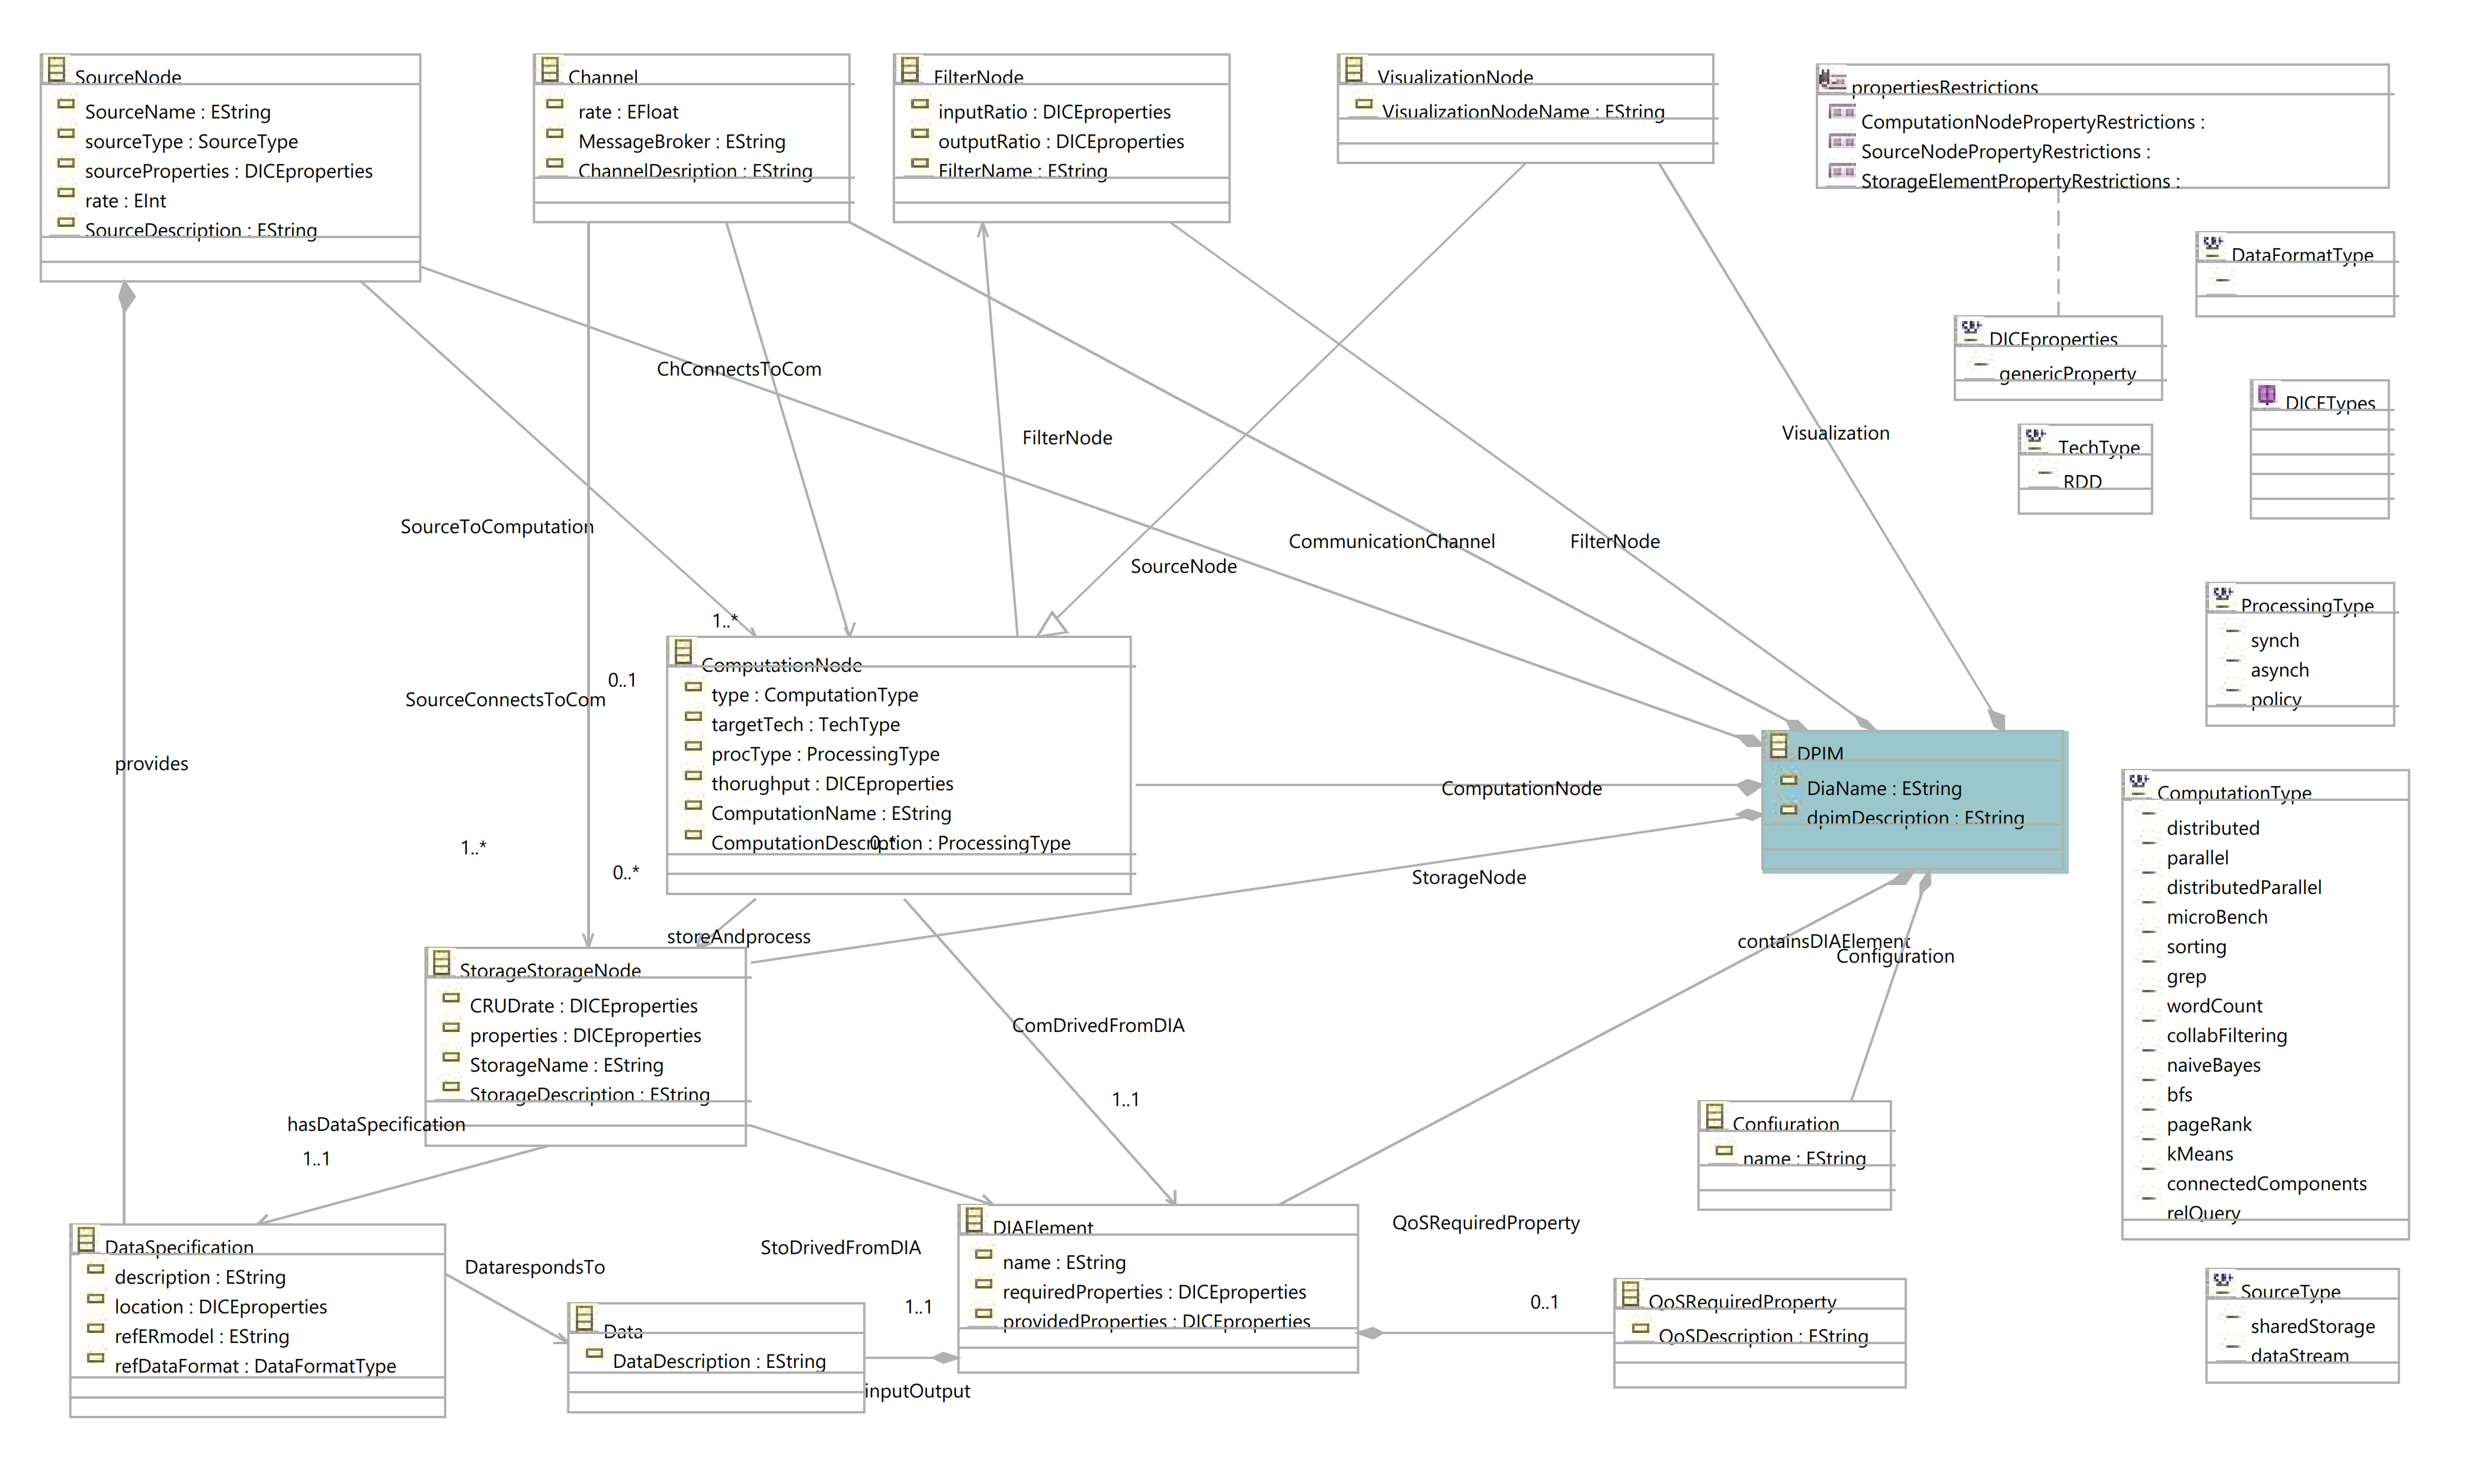
\includegraphics[width=0.8\textwidth]{Images/11.png}
    \caption{High-level Class Diagram}
    \label{fig:class-diagram}
\end{figure}

\subsection{Product Functions}

\subsection{User characteristics}

\subsection{Assumptions, dependencies and constraints}

\subsubsection{Domain Assumptions}
\begin{center}
    {\renewcommand{\arraystretch}{2}
    \begin{tabularx}{\textwidth}{p{2cm} X}
        \hline
        \textbf{ID} & \textbf{Description} \\ \hline
        D1 & Internship descriptions are comprehensive and reliable \\ \hline
        D2 & CVs accurately reflect students' skills and experiences \\ \hline
        D3 & Universities actively oversee internships and intervene when necessary \\ \hline
        D4 & Companies manage interview timelines and conduct them professionally \\ \hline
        D5 & Users provide meaningful feedback to improve the system \\ \hline
        D6 & Problems are reported in a timely manner by all parties \\ \hline
        D7 & The platform supports high user traffic without performance issues \\ \hline 
    \end{tabularx}}
\end{center}
\section{Specific Requirements}

\subsection{External Interface Requirements}

\subsubsection{User interfaces}
\subsubsection{Hardware interfaces}
\subsubsection{Software interfaces}
\subsubsection{Communication interfaces}

\subsection{Functional requirements}

\subsubsection{Requirements}
\subsubsection{Use case diagrams}
\subsubsection{Use case}
\subsubsection{Mapping on goals}

%%
% Alloy language definition for using with the listings package.
%
% 2017, Daniel Andrade
% BSD 3-Clause License
%%
\lstdefinelanguage{alloy}{
    morekeywords={
        module, open, as,
        private, abstract, sig, extends, in,
        lone, some, one, disj,
        fact, pred, fun, assert,
        run, check,
        for, but, exactly,
        this, not, implies, else, let,
        not, no, set, all, sum,
        iff, or, Int, and,
        none, univ, iden
    },
    sensitive=true,
    morecomment=[l]{//},
    morecomment=[l]{--},
    morecomment=[s]{/*}{*/},
    morestring=[b]{"},
%literate={->}{$\rightarrow$}1
% replacing characters can cause problems when copying from PDF to editor
}[keywords,comments,strings]
\section{Effort Spent}

\noindent
\renewcommand{\arraystretch}{1.5}
\setlength{\tabcolsep}{10pt}

\begin{tabularx}{\textwidth}{|>{\columncolor{white}}X|>{\raggedleft\arraybackslash}p{2cm}|}
\hline
\rowcolor{bluepoli!30}
\multicolumn{2}{|c|}{\textbf{Belfiore Mattia}} \\ \hline
\textbf{Section}         & \textbf{Effort (hours)} \\ \hline \hline
Introduction             & -                     \\ \hline
Overall Description      & -                     \\ \hline
Specific Requirements    & -                     \\ \hline
Formal Analysis          & -                     \\ \hline
\rowcolor{bluepoli!20}
\textbf{Total}           & \textbf{-}            \\ \hline
\end{tabularx}

\vspace{1cm} % Aggiungi spazio verticale tra le tabelle

\begin{tabularx}{\textwidth}{|>{\columncolor{white}}X|>{\raggedleft\arraybackslash}p{2cm}|}
\hline
\rowcolor{bluepoli!30}
\multicolumn{2}{|c|}{\textbf{Benedetti Gabriele}} \\ \hline
\textbf{Section}         & \textbf{Effort (hours)} \\ \hline \hline
Introduction             & 5                     \\ \hline
Overall Description      & -                     \\ \hline
Specific Requirements    & -                     \\ \hline
Formal Analysis          & -                     \\ \hline
\rowcolor{bluepoli!20}
\textbf{Total}           & \textbf{5}            \\ \hline
\end{tabularx}

\vspace{1cm} % Aggiungi spazio verticale tra le tabelle

\begin{tabularx}{\textwidth}{|>{\columncolor{white}}X|>{\raggedleft\arraybackslash}p{2cm}|}
\hline
\rowcolor{bluepoli!30}
\multicolumn{2}{|c|}{\textbf{Buccheri Giuseppe}} \\ \hline
\textbf{Section}         & \textbf{Effort (hours)} \\ \hline \hline
Introduction             & 4                     \\ \hline
Overall Description      & -                     \\ \hline
Specific Requirements    & -                     \\ \hline
Formal Analysis          & -                     \\ \hline
\rowcolor{bluepoli!20}
\textbf{Total}           & \textbf{4}            \\ \hline
\end{tabularx}


% Sezione References
\section{References}
\subsection{References}
\subsection{Used Tools}

% Fine del documento
\end{document}
